\documentclass[aspectratio=169,10pt]{beamer}

% Theme
\usetheme{Madrid}
\usecolortheme{whale}

% Packages
\usepackage{booktabs}
\usepackage{graphicx}
\usepackage{listings}
\usepackage{xcolor}
\usepackage{tikz}
\usetikzlibrary{shapes,arrows,positioning,fit,backgrounds}
\usepackage{amsmath}
\usepackage{fontawesome5}

% Colors
\definecolor{codegreen}{rgb}{0.2,0.6,0.2}
\definecolor{codegray}{rgb}{0.5,0.5,0.5}
\definecolor{codepurple}{rgb}{0.58,0,0.82}
\definecolor{backcolour}{rgb}{0.97,0.97,0.97}
\definecolor{pydanticblue}{RGB}{50,100,150}
\definecolor{juliagreen}{RGB}{34,139,34}
\definecolor{posteriorred}{RGB}{178,34,34}
% YAML syntax highlighting colors
\definecolor{yamlkey}{RGB}{0,90,156}       % Blue for keys
\definecolor{yamlstring}{RGB}{163,21,21}   % Red for strings
\definecolor{yamlcomment}{RGB}{106,153,85} % Green for comments
\definecolor{yamlnumber}{RGB}{9,134,88}    % Teal for numbers
\definecolor{yamlkeyword}{RGB}{175,0,219}  % Purple for keywords

% YAML language definition
\lstdefinelanguage{yaml}{
    % Boolean/null keywords
    keywords={true,false,null,yes,no},
    keywordstyle=\color{yamlkeyword}\bfseries,
    % YAML field names (keys) - highlighted in blue
    morekeywords=[2]{
        inputs,name,value,units,input_type,role,source_ref,source_location,
        value_snippet,calibration,parameters,prior,distribution,mu,sigma,
        rationale,model,type,rate_constant,data_rationale,submodel_rationale,
        measurements,observable,state_variables,uses_inputs,evaluation_points,
        sample_size,distribution_code,likelihood,experimental_context,species,
        system,indication,cell_types,phenotype,isolation_method,culture_conditions,
        culture_type,code
    },
    keywordstyle=[2]\color{yamlkey},
    sensitive=false,
    comment=[l]{\#},
    commentstyle=\color{yamlcomment}\itshape,
    stringstyle=\color{yamlstring},
    morestring=[b]",
    morestring=[b]',
}

% Code listings
\lstdefinestyle{yaml}{
    language=yaml,
    backgroundcolor=\color{backcolour},
    basicstyle=\ttfamily\scriptsize,
    breakatwhitespace=false,
    breaklines=true,
    keepspaces=true,
    numbers=none,
    showspaces=false,
    showstringspaces=false,
    showtabs=false,
    tabsize=2,
    frame=single,
    framerule=0.5pt,
    rulecolor=\color{codegray},
    % Colorize structure
    literate=
        *{:}{{{\color{codegray}{:}}}}{1}
        {-}{{{\color{yamlkey}{-}}}}{1}
        {[}{{{\color{codegray}{[}}}}{1}
        {]}{{{\color{codegray}{]}}}}{1},
    % Make keys blue (words before colon)
    moredelim=[is][\color{yamlkey}\bfseries]{<<}{>>},
}

\lstdefinestyle{julia}{
    backgroundcolor=\color{backcolour},
    commentstyle=\color{codegreen},
    keywordstyle=\color{blue},
    numberstyle=\tiny\color{codegray},
    stringstyle=\color{codepurple},
    basicstyle=\ttfamily\scriptsize,
    breakatwhitespace=false,
    breaklines=true,
    keepspaces=true,
    numbers=none,
    showspaces=false,
    showstringspaces=false,
    showtabs=false,
    tabsize=2,
    frame=single,
    framerule=0.5pt,
}

% Title
\title{Automated Calibration Target Extraction \& Joint Bayesian Inference}
\subtitle{QSP-LLM-Workflows Progress Update}
\author{Joel Eliason}
\date{\today}
\institute{Popel Lab}

\begin{document}

\maketitle

% ============================================================================
\section{Overview}
% ============================================================================

\begin{frame}{The Challenge}
\begin{columns}
\begin{column}{0.55\textwidth}
\textbf{Problem:} QSP model calibration requires
\begin{itemize}
    \item Manual extraction of data from papers
    \item Uncertainty quantification for each parameter
    \item Translation to inference code
    \item Validation of extracted values
\end{itemize}
\vspace{0.5em}
\textbf{Current state:} Error-prone, time-consuming, poorly documented
\end{column}
\begin{column}{0.45\textwidth}
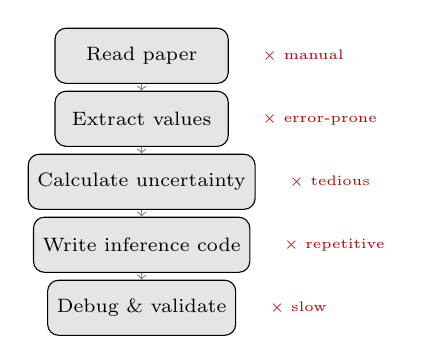
\begin{tikzpicture}[
    taskbox/.style={draw, rounded corners, fill=gray!20, minimum width=2.2cm, minimum height=0.7cm, font=\scriptsize},
]
    \node[taskbox] (read) at (0,2.4) {Read paper};
    \node[taskbox] (extract) at (0,1.6) {Extract values};
    \node[taskbox] (calc) at (0,0.8) {Calculate uncertainty};
    \node[taskbox] (write) at (0,0) {Write inference code};
    \node[taskbox] (debug) at (0,-0.8) {Debug \& validate};

    \draw[->, gray] (read) -- (extract);
    \draw[->, gray] (extract) -- (calc);
    \draw[->, gray] (calc) -- (write);
    \draw[->, gray] (write) -- (debug);

    % Pain points
    \node[right=0.3cm of read, font=\tiny, text=red!70!black] {$\times$ manual};
    \node[right=0.3cm of extract, font=\tiny, text=red!70!black] {$\times$ error-prone};
    \node[right=0.3cm of calc, font=\tiny, text=red!70!black] {$\times$ tedious};
    \node[right=0.3cm of write, font=\tiny, text=red!70!black] {$\times$ repetitive};
    \node[right=0.3cm of debug, font=\tiny, text=red!70!black] {$\times$ slow};
\end{tikzpicture}
\end{column}
\end{columns}
\end{frame}

\begin{frame}{Our Approach: Automated Pipeline}
\begin{center}
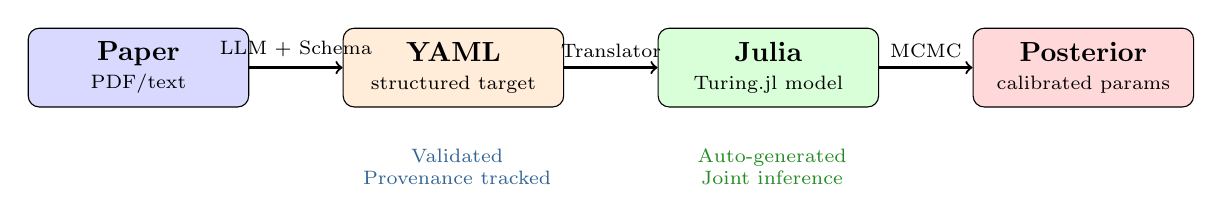
\begin{tikzpicture}[
    box/.style={draw, rounded corners, minimum width=2.8cm, minimum height=1cm, align=center},
    arrow/.style={->, thick},
]
    \node[box, fill=blue!15] (paper) at (0,0) {\textbf{Paper}\\[-2pt]\scriptsize PDF/text};
    \node[box, fill=orange!15] (yaml) at (4,0) {\textbf{YAML}\\[-2pt]\scriptsize structured target};
    \node[box, fill=green!15] (julia) at (8,0) {\textbf{Julia}\\[-2pt]\scriptsize Turing.jl model};
    \node[box, fill=red!15] (posterior) at (12,0) {\textbf{Posterior}\\[-2pt]\scriptsize calibrated params};

    \draw[arrow] (paper) -- (yaml) node[midway, above, font=\scriptsize] {LLM + Schema};
    \draw[arrow] (yaml) -- (julia) node[midway, above, font=\scriptsize] {Translator};
    \draw[arrow] (julia) -- (posterior) node[midway, above, font=\scriptsize] {MCMC};

    % Benefits below
    \node[below=0.4cm of yaml, font=\scriptsize, text=pydanticblue, align=center] {
        $\checkmark$ Validated\\
        $\checkmark$ Provenance tracked
    };
    \node[below=0.4cm of julia, font=\scriptsize, text=juliagreen, align=center] {
        $\checkmark$ Auto-generated\\
        $\checkmark$ Joint inference
    };
\end{tikzpicture}
\end{center}

\vspace{0.5em}
\textbf{Key benefits:}
\begin{itemize}
    \item Pydantic validators catch errors \textit{before} inference
    \item Full provenance: every value traces back to source text
    \item Automatic Julia/Turing.jl code generation with parameter sharing
\end{itemize}
\end{frame}

\begin{frame}{Solution: SubmodelTarget Schema}
\textbf{Key Innovation:} Pydantic schema separating \textit{what} from \textit{how}

\vspace{0.5em}
\begin{center}
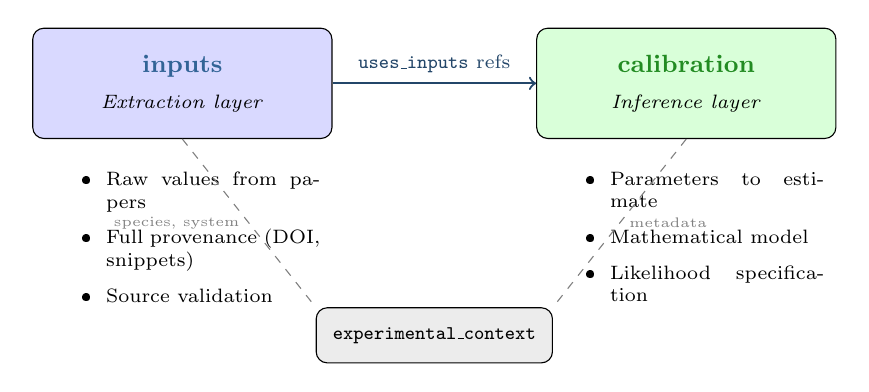
\begin{tikzpicture}[
    box/.style={draw, rounded corners, minimum width=3.8cm, minimum height=1.4cm, align=center, font=\small},
    label/.style={font=\scriptsize, align=left},
]
    % Main boxes - side by side
    \node[box, fill=blue!15] (inputs) at (-3.2,0) {
        \textbf{\textcolor{pydanticblue}{inputs}}\\[2pt]
        \scriptsize\textit{Extraction layer}
    };
    \node[box, fill=green!15] (calib) at (3.2,0) {
        \textbf{\textcolor{juliagreen}{calibration}}\\[2pt]
        \scriptsize\textit{Inference layer}
    };

    % Arrow between them
    \draw[->, thick, pydanticblue!70!black] (inputs) -- (calib)
        node[midway, above, font=\scriptsize] {\texttt{uses\_inputs} refs};

    % Bullet points below each box
    \node[label, below=0.3cm of inputs, anchor=north] {
        \begin{minipage}{3.6cm}
        \begin{itemize}
            \setlength{\itemsep}{1pt}
            \item[\textbullet] Raw values from papers
            \item[\textbullet] Full provenance (DOI, snippets)
            \item[\textbullet] Source validation
        \end{itemize}
        \end{minipage}
    };
    \node[label, below=0.3cm of calib, anchor=north] {
        \begin{minipage}{3.6cm}
        \begin{itemize}
            \setlength{\itemsep}{1pt}
            \item[\textbullet] Parameters to estimate
            \item[\textbullet] Mathematical model
            \item[\textbullet] Likelihood specification
        \end{itemize}
        \end{minipage}
    };

    % Context box below
    \node[draw, rounded corners, fill=gray!15, minimum width=3cm, minimum height=0.7cm, font=\scriptsize]
        (context) at (0,-3.2) {\texttt{experimental\_context}};

    % Dashed lines to context with labels
    \draw[dashed, gray] (inputs.south) -- (context.north west)
        node[midway, left, font=\tiny, text=gray] {species, system};
    \draw[dashed, gray] (calib.south) -- (context.north east)
        node[midway, right, font=\tiny, text=gray] {metadata};
\end{tikzpicture}
\end{center}
\end{frame}

% ============================================================================
\section{Schema Deep Dive}
% ============================================================================

\begin{frame}[fragile]{inputs: Extraction with Provenance}
\begin{lstlisting}[style=yaml]
inputs:
  - name: pdgf_fold_mean
    value: 4.37
    units: dimensionless
    input_type: direct_measurement  # vs proxy, inferred, assumed
    role: target                    # vs auxiliary, initial_condition
    source_ref: Schneider2001_PSC_PDGF
    source_location: Abstract
    value_snippet: "Cell proliferation (4.37 +/- 0.49-fold of control)."

  - name: pdgf_fold_sd
    value: 0.49
    units: dimensionless
    input_type: direct_measurement
    role: auxiliary
    source_ref: Schneider2001_PSC_PDGF
\end{lstlisting}

\textbf{Input types:} \texttt{direct\_measurement}, \texttt{proxy\_measurement}, \texttt{inferred\_estimate}, \texttt{assumed\_value}

\textbf{Roles:} \texttt{target} (in likelihood), \texttt{auxiliary} (supporting), \texttt{initial\_condition} (ODE IC)
\end{frame}

\begin{frame}[fragile]{calibration.parameters: Prior Specification}
\begin{lstlisting}[style=yaml]
calibration:
  parameters:
    - name: k_apsc_prolif
      units: 1/day
      prior:
        distribution: lognormal
        mu: 0.0      # log(1.0) = center at 1/day
        sigma: 1.0   # ~68% between 0.37 and 2.7/day
        rationale: |
          Wide log-normal prior centered at 1/day. A 4-fold increase
          in 1 day implies k ~ ln(4) ~ 1.4/day.
\end{lstlisting}

\textbf{Supported distributions:}
\begin{itemize}
    \item \texttt{lognormal}$(mu, sigma)$ --- positive parameters (rates, concentrations)
    \item \texttt{normal}$(mu, sigma)$ --- unconstrained parameters
    \item \texttt{uniform}$(lower, upper)$ --- bounded parameters
    \item \texttt{half\_normal}$(sigma)$ --- positive with mode at 0
\end{itemize}
\end{frame}

\begin{frame}[fragile]{calibration.model: ODE Model Types}
\begin{columns}
\begin{column}{0.5\textwidth}
\textbf{Built-in ODE models:}
\begin{itemize}
    \item \texttt{exponential\_growth}: $\dot{y} = ky$
    \item \texttt{first\_order\_decay}: $\dot{y} = -ky$
    \item \texttt{two\_state}: $A \xrightarrow{k} B$
    \item \texttt{saturation}: $\dot{y} = k(1-y)$
    \item \texttt{logistic}: $\dot{y} = ky(1-y/K)$
    \item \texttt{michaelis\_menten}: $\dot{y} = -V_{max}y/(K_m+y)$
\end{itemize}
\vspace{0.5em}
\textbf{Non-ODE models:}
\begin{itemize}
    \item \texttt{direct\_conversion}: $k = \ln(2)/t_{1/2}$
    \item \texttt{direct\_fit}: Hill, linear, exponential
    \item \texttt{custom}: user-provided code
\end{itemize}
\end{column}
\begin{column}{0.5\textwidth}
\begin{lstlisting}[style=yaml]
model:
  type: exponential_growth
  rate_constant: k_apsc_prolif
  data_rationale: |
    BrdU assay measures proliferation
    as fold-change over ~24h under
    constant PDGF stimulus.
  submodel_rationale: |
    Full model: k_apsc_prolif * aPSC
    * (PDGF/(PDGF_50 + PDGF))
    At 50 ng/mL PDGF >> PDGF_50,
    reduces to exponential growth.
\end{lstlisting}
\end{column}
\end{columns}
\end{frame}

\begin{frame}[fragile]{calibration.measurements: Likelihood \& Observables}
\begin{lstlisting}[style=yaml]
measurements:
  - name: proliferation_fold_change
    observable:
      type: identity
      state_variables: [aPSC_rel]
    units: dimensionless
    uses_inputs: [pdgf_fold_mean, pdgf_fold_sd]
    evaluation_points: [1.0]  # day
    sample_size: 3
    distribution_code: |
      def derive_distribution(inputs, ureg):
          mean = inputs['pdgf_fold_mean'].magnitude
          sd = inputs['pdgf_fold_sd'].magnitude
          # Monte Carlo to get median and 95% CI
          ...
          return {'median': [4.34], 'ci95': [[3.4, 5.3]], 'units': '...'}
    likelihood:
      distribution: lognormal
      rationale: Fold-changes are positive and multiplicative.
\end{lstlisting}
\end{frame}

\begin{frame}[fragile]{experimental\_context: Metadata for Generalization}
\begin{lstlisting}[style=yaml]
experimental_context:
  species: rat
  system: in_vitro_primary_cells
  indication: PDAC
  cell_types:
    - name: pancreatic stellate cell
      phenotype: activated (alpha-SMA positive)
      isolation_method: Isolated from normal Wistar rat pancreas
  culture_conditions:
    culture_type: 2d_monolayer
\end{lstlisting}

\vspace{0.5em}
\textbf{Why this matters:}
\begin{itemize}
    \item Enables filtering by species/system for meta-analysis
    \item Documents translation assumptions (rat $\rightarrow$ human)
    \item Supports uncertainty inflation for cross-species extrapolation
\end{itemize}
\end{frame}

% ============================================================================
\section{Validators}
% ============================================================================

\begin{frame}{Built-in Pydantic Validators}
\textbf{10 validators} ensure data integrity and prevent hallucinations:

\begin{columns}
\begin{column}{0.5\textwidth}
\textbf{Reference Validation}
\begin{itemize}
    \item \texttt{validate\_input\_refs} --- all \texttt{uses\_inputs} exist
    \item \texttt{validate\_source\_refs} --- all \texttt{source\_ref} match source\_tags
    \item \texttt{validate\_parameter\_roles} --- model params exist
    \item \texttt{validate\_observable\_state\_vars}
\end{itemize}
\end{column}
\begin{column}{0.5\textwidth}
\textbf{Content Validation}
\begin{itemize}
    \item \texttt{validate\_doi\_resolution} --- DOI resolves via CrossRef
    \item \texttt{validate\_input\_values\_in\_snippets} --- anti-hallucination check
    \item \texttt{validate\_units\_are\_valid\_pint}
    \item \texttt{validate\_custom\_code\_syntax} --- AST parsing
    \item \texttt{validate\_span\_ordering}
    \item \texttt{validate\_ode\_model\_requirements}
\end{itemize}
\end{column}
\end{columns}

\vspace{1em}
\begin{block}{Example: Anti-hallucination check}
If \texttt{value\_snippet = "proliferation (4.37 +/- 0.49-fold)"} but \texttt{value = 5.2}, validator raises error.
\end{block}
\end{frame}

% ============================================================================
\section{Julia Translation}
% ============================================================================

\begin{frame}[fragile]{Automatic Julia/Turing.jl Code Generation}
\begin{columns}
\begin{column}{0.55\textwidth}
\textbf{Python YAML:}
\begin{lstlisting}[style=yaml, basicstyle=\ttfamily\tiny]
calibration:
  parameters:
    - name: k_apsc_prolif
      prior:
        distribution: lognormal
        mu: 0.0
        sigma: 1.0
  model:
    type: exponential_growth
    rate_constant: k_apsc_prolif
\end{lstlisting}
\end{column}
\begin{column}{0.45\textwidth}
\textbf{Generated Julia:}
\begin{lstlisting}[style=julia, basicstyle=\ttfamily\tiny]
function ode!(du, u, p, t)
    k_apsc_prolif = p[1]
    du[1] = k_apsc_prolif * u[1]
end

@model function calibration(data)
    # Prior
    k_apsc_prolif ~ LogNormal(0.0, 1.0)

    # Simulate
    sol = solve(ODEProblem(ode!, ...))
    pred = sol[1, end]

    # Likelihood
    data.obs ~ Normal(pred, data.sigma)
end
\end{lstlisting}
\end{column}
\end{columns}

\vspace{0.5em}
\textbf{Key feature:} \textcolor{juliagreen}{Joint inference} --- parameters shared across targets are automatically identified and estimated once.
\end{frame}

\begin{frame}{Joint Inference: Parameter Sharing}
\begin{center}
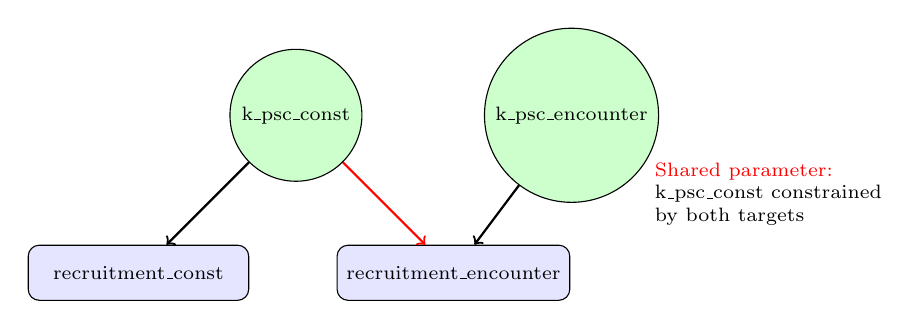
\begin{tikzpicture}[
    target/.style={draw, rounded corners, fill=blue!10, minimum width=2.8cm, minimum height=0.7cm, font=\scriptsize},
    param/.style={draw, circle, fill=green!20, minimum size=1cm, font=\scriptsize},
]
    % Parameters
    \node[param] (kconst) at (0,0) {k\_psc\_const};
    \node[param] (kenc) at (3.5,0) {k\_psc\_encounter};

    % Targets
    \node[target] (rec1) at (-2,-2) {recruitment\_const};
    \node[target] (rec2) at (2,-2) {recruitment\_encounter};

    % Arrows
    \draw[->, thick] (kconst) -- (rec1);
    \draw[->, thick, red] (kconst) -- (rec2);
    \draw[->, thick] (kenc) -- (rec2);

    % Legend
    \node[font=\scriptsize, align=left] at (6, -1) {
        \textcolor{red}{Shared parameter:}\\
        k\_psc\_const constrained\\
        by both targets
    };
\end{tikzpicture}
\end{center}

\vspace{0.5em}
\textbf{10 targets} $\rightarrow$ \textbf{10 parameters} (1 shared: \texttt{k\_psc\_const})

Joint posterior captures correlations and improves identifiability.
\end{frame}

% ============================================================================
\section{Results}
% ============================================================================

\begin{frame}{Joint Inference Results: 10 Parameters}
\begin{table}
\centering
\scriptsize
\begin{tabular}{lrrcc}
\toprule
\textbf{Parameter} & \textbf{Posterior Median} & \textbf{Units} & \textbf{R-hat} & \textbf{ESS} \\
\midrule
k\_ECM\_apsc\_sec & $8.74 \times 10^{-10}$ & mg/(cell$\cdot$day) & 1.001 & 3839 \\
k\_psc\_activation & 2.58 & 1/day & 1.000 & 4074 \\
k\_apsc\_death & 0.091 & 1/day & 1.002 & 4020 \\
k\_qpsc\_death & 0.178 & 1/day & 1.002 & 3802 \\
k\_apsc\_prolif & 1.44 & 1/day & 1.001 & 4590 \\
k\_psc\_const & $3.49 \times 10^{7}$ & cell/mL & 1.002 & 2670 \\
k\_psc\_encounter & $2.54 \times 10^{5}$ & cell/(mL$\cdot$day) & 1.001 & 2388 \\
p\_T\_kill\_per\_contact & 0.150 & -- & 1.000 & 4023 \\
k\_TGFb\_sec\_apsc & $3.75 \times 10^{-10}$ & nM$\cdot$L/(cell$\cdot$day) & 1.002 & 3282 \\
\textbf{R50\_Treg} & \textbf{0.411} & -- & 1.000 & 4571 \\
\bottomrule
\end{tabular}
\end{table}

\vspace{0.5em}
\textbf{All parameters converged:} R-hat $\approx$ 1.0, ESS $>$ 2000

\textbf{New target:} R50\_Treg (Treg:Teff ratio for 50\% suppression) = 0.41
\end{frame}

\begin{frame}{Posterior Predictive Diagnostics}
\begin{table}
\centering
\scriptsize
\begin{tabular}{lrrrcc}
\toprule
\textbf{Target} & \textbf{Observed} & \textbf{Predicted} & \textbf{Z-score} & \textbf{90\%} & \textbf{95\%} \\
\midrule
ecm\_secretion\_apsc & $6.48 \times 10^{-10}$ & $8.74 \times 10^{-10}$ & $-0.69$ & \checkmark & \checkmark \\
psc\_activation\_rate & 0.950 & 0.994 & $-1.19$ & \checkmark & \checkmark \\
psc\_death\_activated & 0.086 & 0.078 & 0.38 & \checkmark & \checkmark \\
psc\_death\_quiescent & 0.198 & 0.178 & 0.42 & \checkmark & \checkmark \\
psc\_proliferation & 4.34 & 4.23 & 0.22 & \checkmark & \checkmark \\
psc\_recruitment\_const & $3.72 \times 10^{7}$ & $3.49 \times 10^{7}$ & 0.15 & \checkmark & \checkmark \\
tcell\_kill\_probability & 0.150 & 0.150 & $-0.01$ & \checkmark & \checkmark \\
tgfb\_secretion\_apsc & $4.25 \times 10^{-10}$ & $3.75 \times 10^{-10}$ & 0.27 & \checkmark & \checkmark \\
treg\_suppression\_r50 & 0.507 & 0.411 & 0.66 & \checkmark & \checkmark \\
\bottomrule
\end{tabular}
\end{table}

\vspace{0.5em}
\begin{columns}
\begin{column}{0.5\textwidth}
\textbf{Summary Statistics:}
\begin{itemize}
    \item Mean $|Z|$ = 0.44 (ideal: $<$1.0) \textcolor{green}{\checkmark}
    \item Max $|Z|$ = 1.19 (ideal: $<$2.0) \textcolor{green}{\checkmark}
    \item RMSE = 0.56 (ideal: $\sim$1.0) \textcolor{green}{\checkmark}
\end{itemize}
\end{column}
\begin{column}{0.5\textwidth}
\textbf{Posterior Coverage:}
\begin{itemize}
    \item 90\% CI: 100\% coverage (expected: 90\%)
    \item 95\% CI: 100\% coverage (expected: 95\%)
\end{itemize}
$\rightarrow$ Well-calibrated uncertainties
\end{column}
\end{columns}
\end{frame}

% ============================================================================
\section{Summary}
% ============================================================================

\begin{frame}{Summary \& Next Steps}
\textbf{What we built:}
\begin{itemize}
    \item \textbf{SubmodelTarget} --- Pydantic schema separating extraction from inference
    \item \textbf{10 built-in validators} --- DOI resolution, anti-hallucination, unit checking
    \item \textbf{Julia translator} --- Automatic Turing.jl code generation with joint inference
    \item \textbf{10 calibration targets} for PDAC stromal biology
\end{itemize}

\vspace{0.5em}
\textbf{Results:}
\begin{itemize}
    \item All 10 parameters converged (R-hat $\approx$ 1.0)
    \item Excellent posterior predictive metrics (mean $|Z|$ = 0.44, 100\% coverage)
    \item New target: R50\_Treg = 0.41 (Treg suppression)
\end{itemize}

\vspace{0.5em}
\textbf{Next steps:}
\begin{itemize}
    \item Expand to full PDAC immune module (CD8, MDSC, macrophages)
    \item LLM-assisted extraction pipeline with human-in-the-loop
    \item Integration with full QSP model for virtual population generation
\end{itemize}
\end{frame}

\begin{frame}
\begin{center}
\Huge Questions?

\vspace{1em}
\normalsize
Code: \texttt{github.com/popellab/qsp-llm-workflows}
\end{center}
\end{frame}

\end{document}
